\section{Examples of the Morse complex} \label{section:morse_examples}

In this section we are going to provide some examples of the Morse complexes constructed in various manifolds these examples are meant to illustrate the properties of the Morse homology, as well as give some sense to how the theory is developed.

\subsection{The sphere}

\begin{exmpl}
Consider the 2 dimensional sphere embedded inside $\R^3$ and the height function $h(x,y,z) = z$ (restricted to $\con{S}^2$). As we saw in \ref{coro:reeb}, the spheres are the only compact manifolds without boundary that admit only two critical points, and the height function is the prime example of this.

\begin{figure}[h] \label{figure:example1}
	\centering
	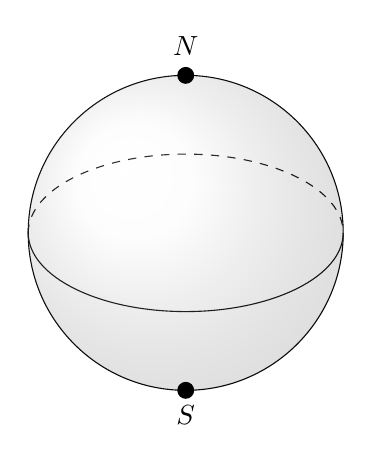
\begin{tikzpicture}
	\draw (-2,0) arc (180:360:2cm and 1cm);
	\draw[dashed] (-2,0) arc (180:0:2cm and 1cm);
	\draw (0,0) circle (2cm);
	\shade[ball color=gray!10!white,opacity=0.20] (0,0) circle (2cm);
	\draw [fill] (0,2) circle [radius=0.1cm]
	node [label={[above]$N$}] {};
	\draw [fill] (0,-2) circle [radius=0.1cm]
	node [label={[below,yshift=-0.2cm]$S$}] {};
\end{tikzpicture}
	\caption{The critical points of $h$ on $\con{S}^2$.}
\end{figure}

In this case (see figure \ref{figure:example1}), the complex is easy to construct. The only critical points of $h$ are $S$ (of index 0) and $N$ of index 2, and the vector field $- \grad h$ (defined using the euclidean metric) satisfies the Smale condition, so we can use it to define the differential of the complex. However, we just commented that
\[C_k(\con{S}^2,h) = \left\{ \begin{array}{lc} \con{Z}_2 S & \text{if } k=0 \\ \con{Z}_2 N & \text{if } k=2 \\ 0 & \text{otherwise} \end{array} \right. ,\]
so $\partial_k = 0$ for all $k$. Therefore, the homology that results is the one that we might expect:
\[H_k(\con{S}^2,h) = \left\{ \begin{array}{lc} \con{Z}_2 & \text{if } k=0,2 \\ 0 & \text{otherwise} \end{array} \right. .\]
\end{exmpl}

\begin{exmpl} Allow us to show a different function on the sphere. This function, $f$ is such that it induces the dynamics shown in Figure \ref{figure:example2}. In particular, it has the following critical points:
\begin{itemize}
	\item The local maxima $a_1,a_2$ and $a_3$, which are critical points of index $2$.
	\item The critical points $b_1$ and $b_2$ of index $1$.
	\item The absolute minimum $c$, of index $0$.
\end{itemize}

\begin{figure}[h] \label{figure:example2}
	\centering
	\begin{tikzpicture}
	%Sphere
	\draw (-3,0) arc (180:360:3cm and 1.5cm);
	\draw[dashed] (-3,0) arc (180:0:3cm and 1.5cm);
	\draw (0,0) circle (3cm);
	\shade[ball color=gray!10!white,opacity=0.20] (0,0) circle (3cm);

	%Point a_1
	\draw [fill] (0,3) circle [radius=0.75mm]
	node [label={[above]$a_1$}] {};
	%Point a_2
	\draw [fill] (-2,-1.5) circle [radius=0.75mm]
	node [label={[below,xshift=3mm,yshift=-2mm]$a_2$}] {};
	%Point a_3
	\draw [fill=gray!90!white,draw=gray!90!white] (2,-1.5) circle [radius=0.75mm]
	node [label={[below,xshift=-3mm,yshift=-2mm]$a_3$}] {};
	%Point b_1
	\draw [fill] (-2,1.5) circle [radius=0.75mm]
	node [label={[above,xshift=-0.5mm,yshift=-0.6mm]$b_1$}] {};
	%Point b_2
	\draw [fill=gray!90!white,draw=gray!90!white] (2,1.5) circle [radius=0.75mm]
	node [label={[above,yshift=-0.6mm,xshift=1mm]$b_2$}] {};
	%Point c
	\draw [fill] (0,-3) circle [radius=0.75mm]
	node [label={[below,yshift=-0.2cm]$c$}] {};

	%Trajectory from a_1 to b_1
	\draw[-{Latex[length=2mm]}] (0,3) to [out=190,in=40] (-1.3,2.4);
	\draw[] (-1.2,2.5) to [out=220,in=60] (-2,1.5);

	%Trajectory from a_1 to b_2
	\draw[-{Latex[length=2mm]},dashed] (0,3) to [out=350,in=140] (1.3,2.4);
	\draw[dashed] (1.2,2.5) to [out=320,in=120] (1.95,1.6);

	%Trajectory from a_2 to b_1
	\draw[-{Latex[length=2mm]}] (-2,-1.5) to [out=120,in=275] (-2.4,-0.4);
	\draw[] (-2.4,-0.45) to [out=95,in=240] (-2,1.5);

	%Trajectory from a_3 to b_2
	\draw[-{Latex[length=2mm]},dashed] (2,-1.5) to [out=60,in=265] (2.4,-0.4);
	\draw[dashed] (2.4,-0.45) to [out=85,in=300] (2.05,1.4);

	%Trajectory from b_1 to c
	\draw[-{Latex[length=2mm]}] (-2,1.5) to [out=330,in=110] (-0.49,-0.51);
	\draw[] (-0.5,-0.5) to [out=290,in=100] (0,-3);

	%Trajectory from b_2 to c
	\draw[-{Latex[length=2mm]},dashed] (2,1.5) to [out=210,in=70] (0.5,-0.5);
	\draw[dashed] (0.5,-0.5) to [out=250,in=80] (0,-3);

	%Trajectory from b_1 to c (behind)
	\draw[] (-2,1.5) to [out=150,in=80.41] (-2.96,0.5);
	\draw[-{Latex[length=2mm]},dashed] (-2.96,0.5) to [out=260.41,in=150] (-1.1,-2.6);
	\draw[dashed] (-1.1,-2.6) to [out=330,in=165] (0,-3);

	%Trajectory from b_2 to c (in front)
	\draw[dashed] (2,1.5) to [out=30,in=99.59] (2.96,0.5);
	\draw[-{Latex[length=2mm]}] (2.96,0.5) to [out=279.59,in=30] (1.05,-2.63);
	\draw[] (1.1,-2.6) to [out=210,in=15] (0,-3);
\end{tikzpicture}

	\caption{The critical points and some trajectories of function $f$ over $\con{S}^2$.}
\end{figure}

In Figure \ref{figure:example2} we sketch the dynamics induced by this function by plotting the trajectories that connect critical points of consecutive indices (one has to imagine that all the points of $\con{S}^2$ not belonging to any of these trajectories belong to a trajectory connecting a critical point of index $2$ to $c$).

Therefore, we already know that
\[C_k(\con{S}^2,f) = \left\{ \begin{array}{lc} \langle a_1, a_2, a_3 \rangle_{\con{Z}_2} & \text{if } k=2 \\ \langle b_1,b_2\rangle_{\con{Z}_2} & \text{if } k=1 \\ \langle c \rangle_{\con{Z}_2} & \text{if } k=0 \end{array} \right. ,\]
this means, $C_2(\con{S}^2,f) \cong \con{Z}_2^3$, $C_1(\con{S}^2,f) \cong \con{Z}_2^2$ and $C_0(\con{S}^2,f) \cong \con{Z}_2$.

Moreover, we can compute the differential over the generators of each group of the complex:
\[\partial_2 a_1 = b_1+b_2 \, , \, \partial_2 a_2 = b_1 \, , \, \partial_2 a_3 = b_2,\]
\[\partial_1 b_1 = 2c = 0 \, , \, \partial_1 b_2 = 2c = 0 .\]
From this, we deduce that $\partial_1 = 0$, and
\[\partial_2 = \begin{pmatrix} 1 & 1 & 0 \\ 1 & 0 & 1 \end{pmatrix} .\]
This means, $\text{Im}(\partial_2) = C_1(\con{S}^2,f)$, and $\text{Ker}(\partial_2) = \langle a_1+a_2+a_3 \rangle_{\con{Z}_2}$. This gives us a complete description of the homology groups:
\[H_0(\con{S}^2,f) = \quocient{C_0(\con{S}^2,f)}{\text{Im}(\partial_1)} = \con{Z}_2[c] ,\]
\[H_1(\con{S}^2,f) = \quocient{\text{Ker}(\partial_1)}{\text{Im}(\partial_2)} = \quocient{C_1(\con{S}^2,f)}{C_1(\con{S}^2,f)} = 0,\]
\[H_2(\con{S}^2,f) = \quocient{\text{Ker}(\partial_2)}{0} = \con{Z}_2 [a_1+a_2+a_3] .\]

In particular, it is clear that $H_k(\con{S}^2,h) \cong H_k(\con{S}^2,f)$, suggesting that (as we will prove in Section \ref{section:morse_well_defined}) the homology of a manifold does not depend on the function used to define it.
\end{exmpl}

\subsection{The torus}


